\subsection{Create a table of descriptive statistics of the variables in the dataset.}
% latex table generated in R 4.2.1 by xtable 1.8-4 package
% Wed Dec  6 21:45:13 2023
\begin{table}[ht]
\centering
\begin{tabular}{llllllr}
  \hline
var & median & mean & min & max & sd & NAs \\ 
  \hline
agro\_emp & 18.6 & 25.1 & 0.1 & 86.3 & 22.3 &  30 \\ 
  bribery & 11.7 & 17.0 & 0.0 & 67.1 & 14.7 &  87 \\ 
  gfce & 16.5 & 17.7 & 5.1 & 62.9 & 8.4 &  36 \\ 
  literacy & 93.0 & 83.6 & 24.2 & 100.0 & 19.3 &  61 \\ 
  log\_gdp & 9.4 & 9.3 & 6.6 & 11.6 & 1.2 &  22 \\ 
  pop\_total & 6.2e+06 & 3.4e+07 & 1.1e+04 & 1.4e+09 & 1.4e+08 &   2 \\ 
  self\_emp & 35.0 & 40.9 & 0.4 & 94.8 & 27.0 &  30 \\ 
  stocks & 6.4 & 28.8 & 0.0 & 538.7 & 66.8 & 131 \\ 
  sample\_size & 715.1 & 3.6e+03 & 120.1 & 1.4e+05 & 1.3e+04 &   2 \\ 
   \hline
\end{tabular}
\caption{Descriptive statistics} 
\label{desc}
\end{table}



The data is made of 217 countries and certain variables contains a significant
amount of missing values (NAs) (See \ref{desc}). Bribery is the worst variable with up to 87 NAs. Using
this variable in a regression would yield a low precision as the size of the sample is quite small.
This table demonstrates how different countries are, indeed the min-max interval is rather close to one for rate variables and the standart deviations (sd)
are very significant compared to the mean value of each variable.

\stepcounter{subsection}
\subsubsection{Is it the case that self-employment is correlated with how rich a country is (in-terms of log GDP per-capita)?}


\begin{figure}[htbp]
  \centering
  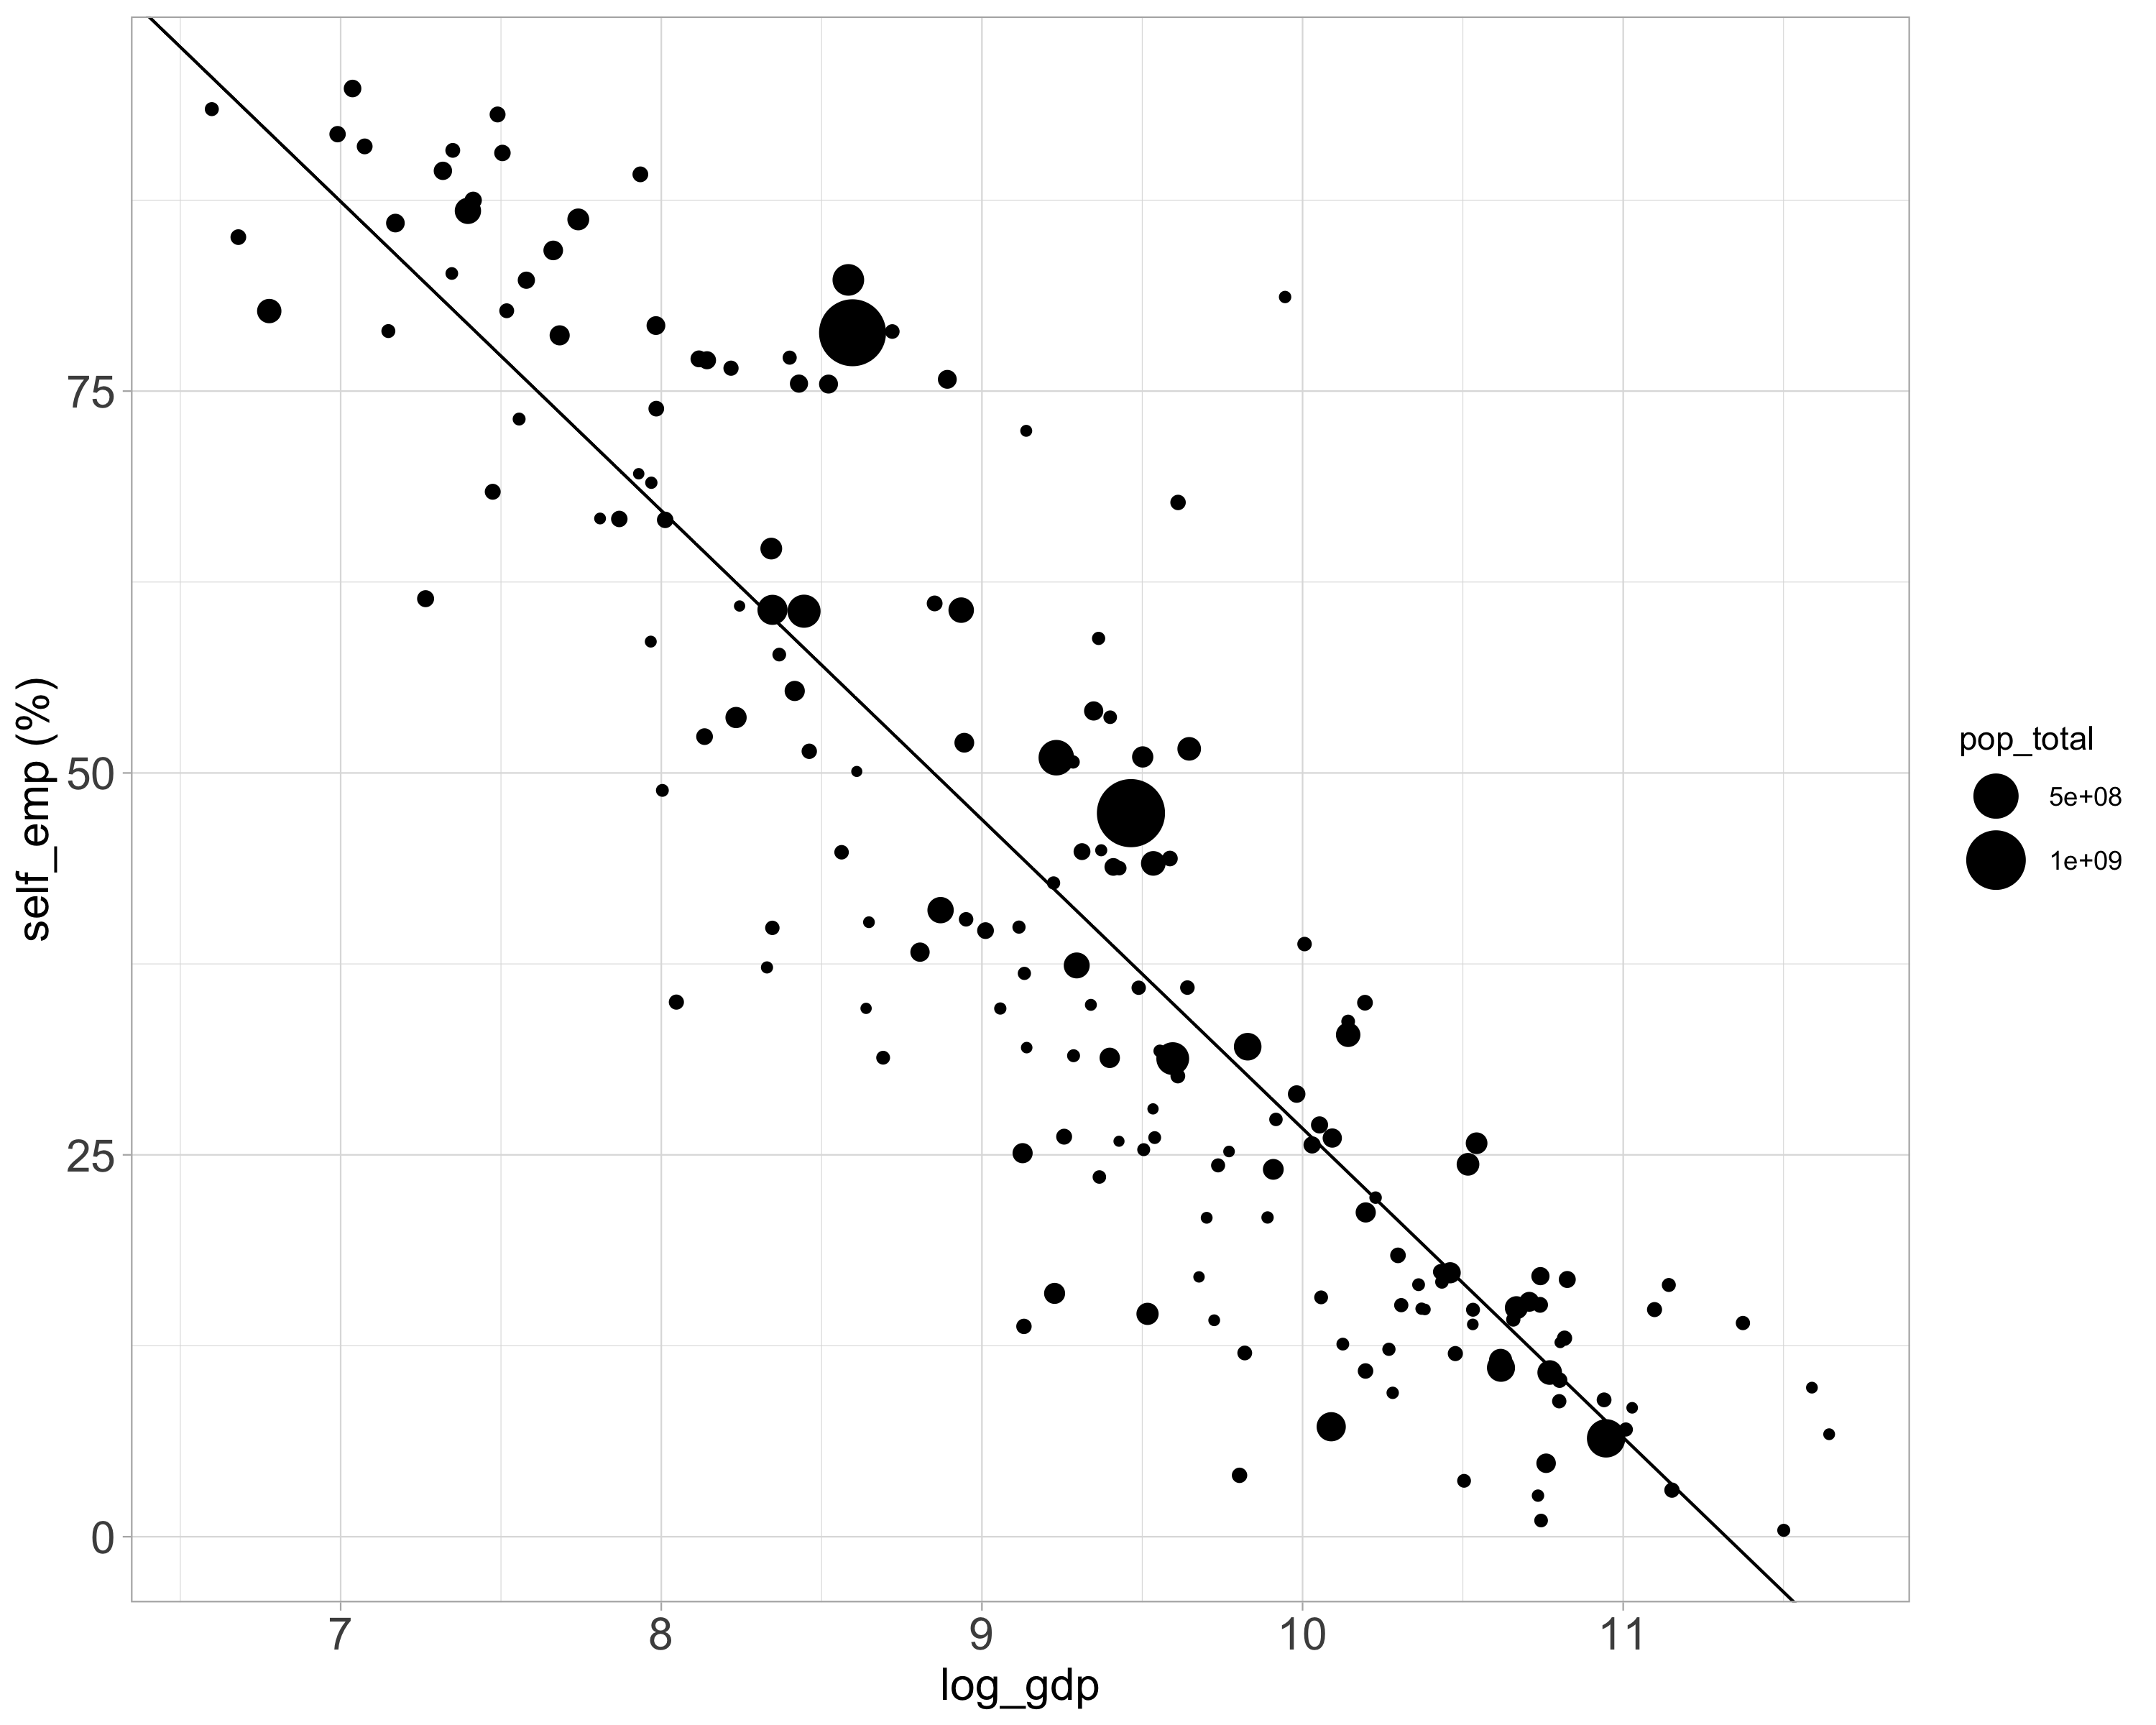
\includegraphics[width=0.8\textwidth]{Exercise_1/OUTPUT/emp_wrt_gdp.png}
  \caption{Self employment rate with respect to GDP}
  \label{fig:emp_gdp}
\end{figure}


Figure \ref{fig:emp_gdp} shows a clear negative relationship between the share of self employment and gdp. The empirical correlation coefficient is equal to $-0.89$
which is very close to $-1$. The anticorrelation is very strong.
\subsubsection{Is it the case that countries with higher share of employment in agriculture also have higher self-employment rates?}

\begin{figure}[htbp]
  \centering
  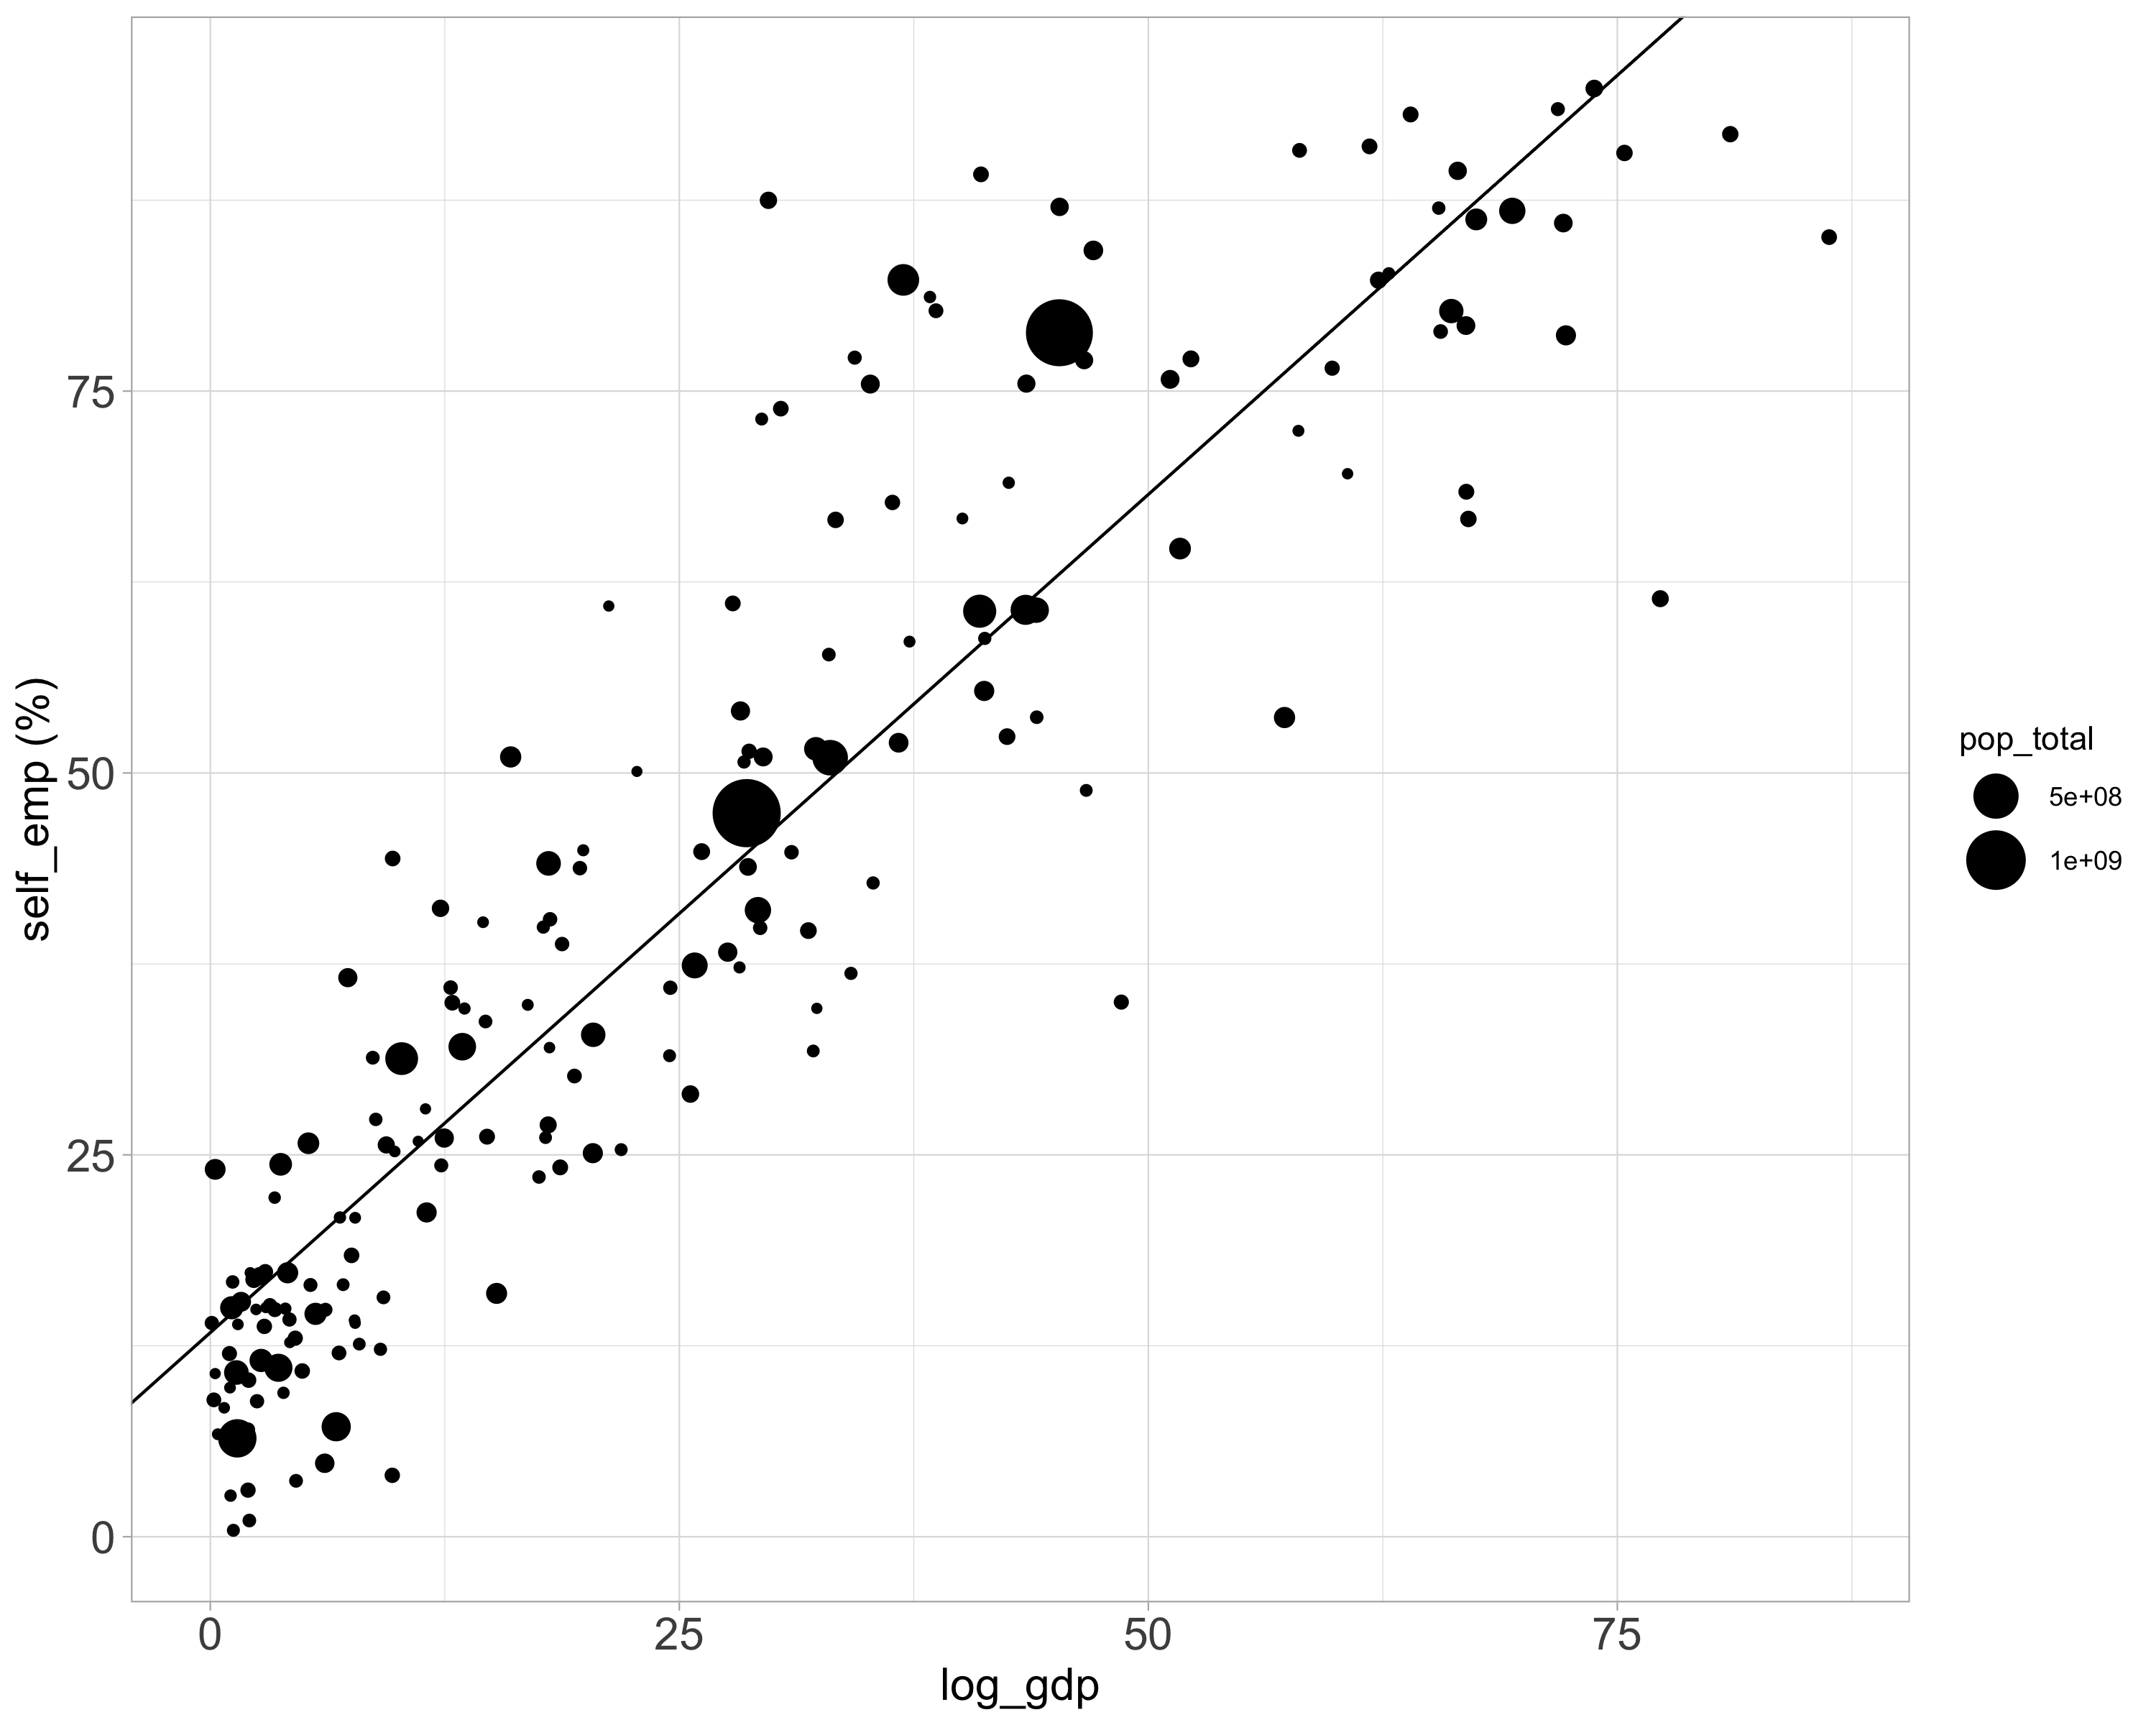
\includegraphics[width=0.8\textwidth]{Exercise_1/OUTPUT/emp_wrt_agro.png}
  \caption{Self employment rate with respect to employment share in the agricultural sector}
  \label{fig:emp_agro}
\end{figure}

As in the previous question, Figure \ref{fig:emp_agro} shows a clear positive relationship between the share of self employment and share of employment in the agricultural sector. The empirical correlation coefficient is equal to $0.91$
which is very close to $1$. The correlation is very strong.

\subsubsection{Present a bar graph comparing the mean self-employment rates in each of these 3 literacy-based categories of countries.}
\begin{figure}[htbp]
  \centering
  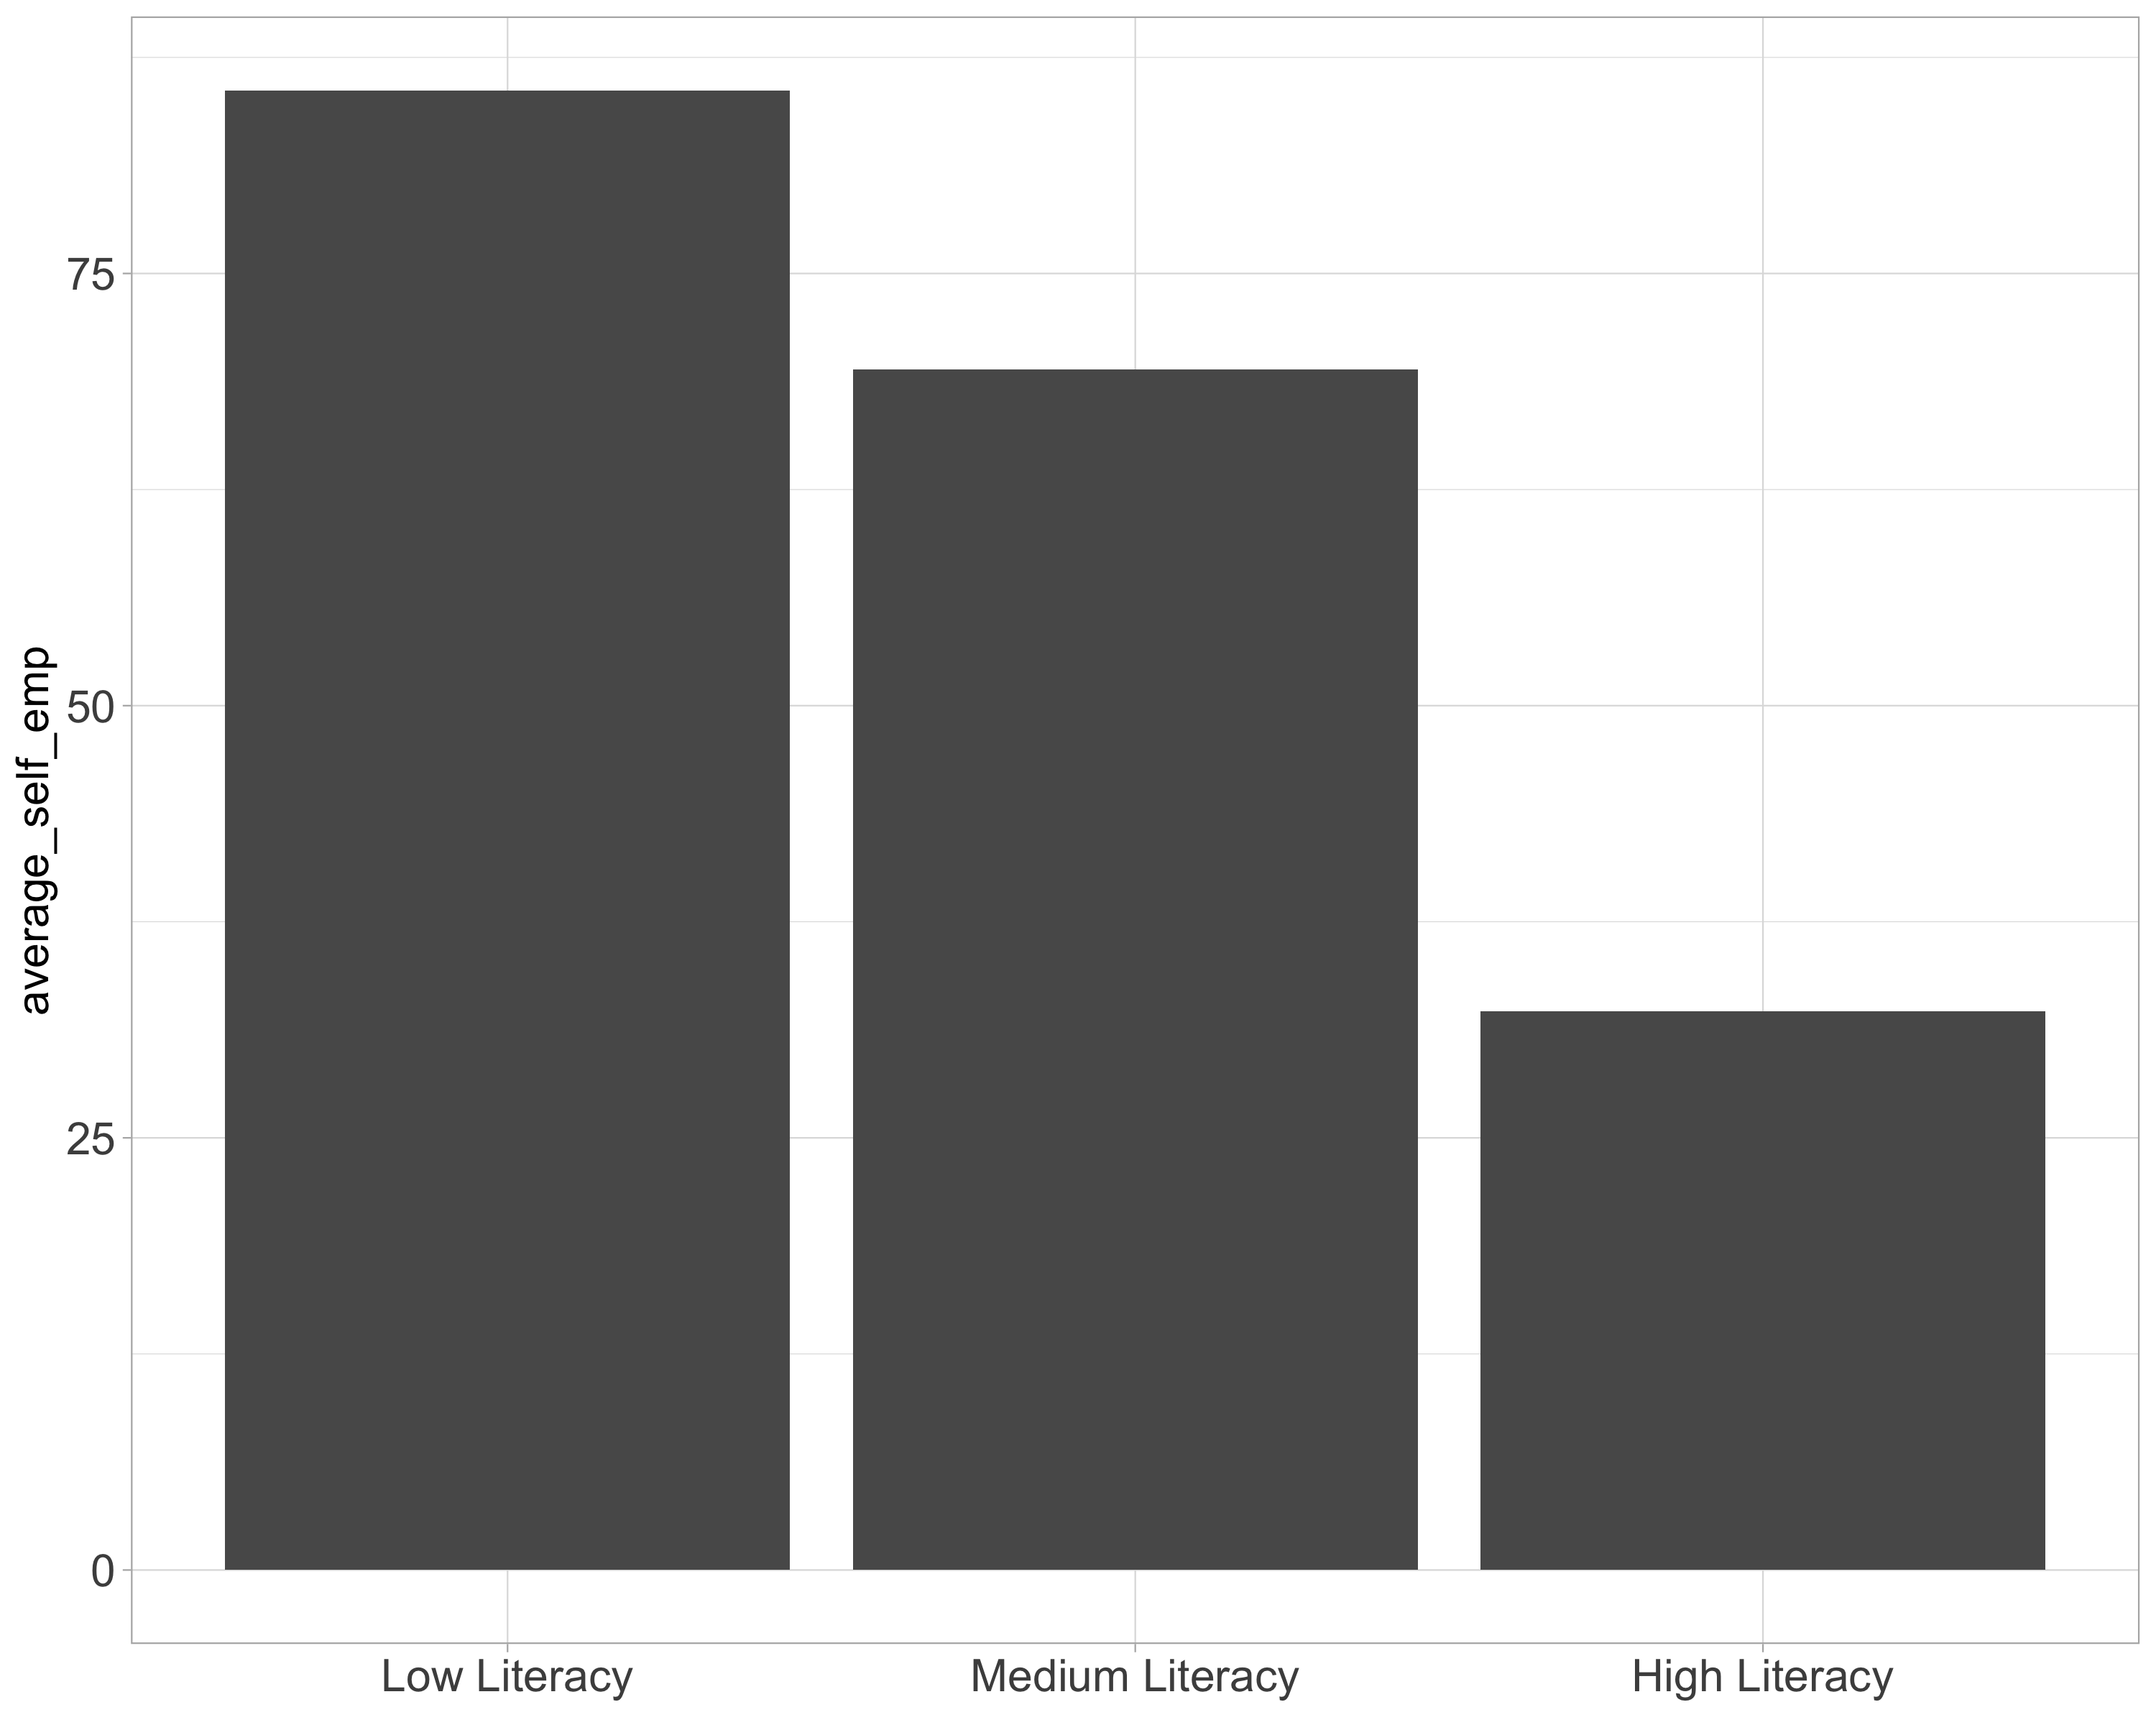
\includegraphics[width=0.8\textwidth]{Exercise_1/OUTPUT/bar_emp_literacy.png}
  \caption{Average self employement rate as a function of the literacy category}
  \label{fig:emp_lit}
\end{figure}

Figure \ref{fig:emp_lit} seems to demonstrate a negative relationship between the literacy category of the population and the self employment rate.

\subsection{Estimate the model parameters described using OLS, report your results and summarize them}

% Table created by stargazer v.5.2.3 by Marek Hlavac, Social Policy Institute. E-mail: marek.hlavac at gmail.com
% Date and time: Jeu, déc 07, 2023 - 11:24:15
% Requires LaTeX packages: dcolumn 
\begin{table}[!htbp] \centering 
  \caption{Linear Regressions - Exercise 1} 
  \label{results_1} 
\begin{tabular}{@{\extracolsep{5pt}}lD{.}{.}{-3} D{.}{.}{-3} } 
\\[-1.8ex]\hline 
\hline \\[-1.8ex] 
 & \multicolumn{2}{c}{\textit{Dependent variable:}} \\ 
\cline{2-3} 
\\[-1.8ex] & \multicolumn{2}{c}{self\_emp} \\ 
\\[-1.8ex] & \multicolumn{1}{c}{(1)} & \multicolumn{1}{c}{(2)}\\ 
\hline \\[-1.8ex] 
 log\_gdp & -6.506^{***} & -5.520 \\ 
  & (1.755) & (4.042) \\ 
  & & \\ 
 literacy & -0.313^{***} & -0.358^{**} \\ 
  & (0.070) & (0.175) \\ 
  & & \\ 
 agro\_emp & 0.592^{***} & 0.628^{***} \\ 
  & (0.080) & (0.176) \\ 
  & & \\ 
 gfce &  & -0.922^{**} \\ 
  &  & (0.380) \\ 
  & & \\ 
 stocks &  & 0.110^{*} \\ 
  &  & (0.061) \\ 
  & & \\ 
 bribery &  & -0.111 \\ 
  &  & (0.156) \\ 
  & & \\ 
 Constant & 113.219^{***} & 121.953^{***} \\ 
  & (16.361) & (41.265) \\ 
  & & \\ 
\hline \\[-1.8ex] 
Observations & \multicolumn{1}{c}{143} & \multicolumn{1}{c}{49} \\ 
R$^{2}$ & \multicolumn{1}{c}{0.845} & \multicolumn{1}{c}{0.828} \\ 
Adjusted R$^{2}$ & \multicolumn{1}{c}{0.841} & \multicolumn{1}{c}{0.804} \\ 
Residual Std. Error & \multicolumn{1}{c}{10.574 (df = 139)} & \multicolumn{1}{c}{9.262 (df = 42)} \\ 
F Statistic & \multicolumn{1}{c}{252.152$^{***}$ (df = 3; 139)} & \multicolumn{1}{c}{33.720$^{***}$ (df = 6; 42)} \\ 
\hline 
\hline \\[-1.8ex] 
\textit{Note:}  & \multicolumn{2}{r}{$^{*}$p$<$0.1; $^{**}$p$<$0.05; $^{***}$p$<$0.01} \\ 
\end{tabular} 
\end{table} 

Denoting this linear model as (1) (we shall refer to it as the "simple estimation" in the rest of this section) and estimating it yields the results displayed in Table \ref{results_1} (first column).
This OLS estimation was based on only 143 observations, which is far from 217. This raises a
question, are NAs equally distributed across the sample ? That being aknowledged, this regression seems
to be very significant. The overall significance is very high as the F-stat demonstrates.
Every of the three coefficients are significantly different from zero at the 1\% level.
The signs of the variables are in line with the previous discussion in question 1.1.
According to this estimation, a 1\% increase in GDP corresponds to a 6.5\% decrease in the share of self employement.
A 1\% increase in the literacy rate is associated with a 0.3\% decrease in the dependent variable, while a 0.59\% increase in self employment shares 
can be explained by a 1\% increase in the share of the agricultural sector.

\subsection{Describe how you could estimate $\beta_3$ using a 3-step procedure based on the Frisch-Waugh Theorem.}
The Frisch-Waugh theorem can be used for estimating specific coefficients in a multiple regression model while controlling for other variables. Here are the simplified three steps:


\textbf{Step 1:}\\
Identify control variables, here log\_gdp and literacy, and regress it on the dependent variable to get the residuals $\hat{r}$. The residuals of this regression is the part of self\_emp that is not explained by the log\_gdp and literacy variables.
\begin{equation*}
  \text{self\_emp} = \alpha_0 + \alpha_1 \text{log\_gdp} + \alpha_2 \text{literacy} + r 
\end{equation*}
\textbf{Step 2:}\\
Regress the variable of interest on the control variables and get the residuals $\hat{u}$. The residuals of this regression is the part of agro\_emp that is not explained by the log\_gdp and literacy variables.
\begin{equation*}
  \text{agro\_emp} = \gamma_0 + \gamma_1 \text{log\_gdp} + \gamma_2 \text{literacy} + u 
\end{equation*}
\textbf{Step 3:}\\
Regress $\hat{r}$ on $\hat{u}$ and get the coefficient of interest $\beta_3$. 
\begin{equation*}
  \hat{r} = \beta_0 + \beta_3 \hat{u} + \epsilon
\end{equation*}
The coefficient $\beta_3$ is the estimate of the parameter for agro\_emp after controlling for log\_gdp and literacy.

\subsection{Implement this 3-step procedure and compare your estimate and standard error of $\beta_3$.}
Table \ref{step_1_2_results} and Table \ref{step_3_results} display the results of the 3-step
procedure previously described,
where $\hat{r}$, $\hat{u}$ are respectively denoted as r\_hat and u\_hat.
The first regression yields coefficients that are very different from the first estimation (first column of Table \ref{results_1}).
This is an expected result, indeed as agro\_emp is assumed to be part of the data generating process,
the first step estimation is inconsistent because of endogeneity issues.
The higher the correlation between agro\_emp and control variable, the larger is the discrepency between coefficients from the first step of the Frisch-Waugh procedure and the simple estimation.
The third regression yields an estimation for $\beta_3$ and its standard error which are very close to what we got in the simple estimation.
Those results were expected and a direct implication of the Frisch-Waugh theorem. 

% Table created by stargazer v.5.2.3 by Marek Hlavac, Social Policy Institute. E-mail: marek.hlavac at gmail.com
% Date and time: Jeu, déc 07, 2023 - 20:29:30
% Requires LaTeX packages: dcolumn 
\begin{table}[!htbp] \centering 
  \caption{First and Second Regressions in 3-step Procedure - Exercise 1} 
  \label{step_1_2_results} 
\small 
\begin{tabular}{@{\extracolsep{5pt}}lD{.}{.}{-3} D{.}{.}{-3} } 
\\[-1.8ex]\hline 
\hline \\[-1.8ex] 
 & \multicolumn{2}{c}{\textit{Dependent variable:}} \\ 
\cline{2-3} 
\\[-1.8ex] & \multicolumn{1}{c}{self\_emp} & \multicolumn{1}{c}{agro\_emp} \\ 
\\[-1.8ex] & \multicolumn{1}{c}{(1)} & \multicolumn{1}{c}{(2)}\\ 
\hline \\[-1.8ex] 
 log\_gdp & -15.784^{***} & -15.670^{***} \\ 
  & (1.453) & (1.308) \\ 
  & & \\ 
 literacy & -0.377^{***} & -0.108 \\ 
  & (0.081) & (0.073) \\ 
  & & \\ 
 Constant & 219.877^{***} & 180.127^{***} \\ 
  & (9.247) & (8.326) \\ 
  & & \\ 
\hline \\[-1.8ex] 
Observations & \multicolumn{1}{c}{143} & \multicolumn{1}{c}{143} \\ 
R$^{2}$ & \multicolumn{1}{c}{0.783} & \multicolumn{1}{c}{0.743} \\ 
Adjusted R$^{2}$ & \multicolumn{1}{c}{0.780} & \multicolumn{1}{c}{0.739} \\ 
Residual Std. Error (df = 140) & \multicolumn{1}{c}{12.454} & \multicolumn{1}{c}{11.215} \\ 
F Statistic (df = 2; 140) & \multicolumn{1}{c}{252.747$^{***}$} & \multicolumn{1}{c}{201.952$^{***}$} \\ 
\hline 
\hline \\[-1.8ex] 
\textit{Note:}  & \multicolumn{2}{r}{$^{*}$p$<$0.1; $^{**}$p$<$0.05; $^{***}$p$<$0.01} \\ 
\end{tabular} 
\end{table} 


% Table created by stargazer v.5.2.3 by Marek Hlavac, Social Policy Institute. E-mail: marek.hlavac at gmail.com
% Date and time: Jeu, déc 07, 2023 - 20:29:30
% Requires LaTeX packages: dcolumn 
\begin{table}[!htbp] \centering 
  \caption{Third Regression in 3-step Procedure - Exercise 1} 
  \label{step_3_results} 
\small 
\begin{tabular}{@{\extracolsep{5pt}}lD{.}{.}{-3} } 
\\[-1.8ex]\hline 
\hline \\[-1.8ex] 
 & \multicolumn{1}{c}{\textit{Dependent variable:}} \\ 
\cline{2-2} 
\\[-1.8ex] & \multicolumn{1}{c}{r\_hat} \\ 
\hline \\[-1.8ex] 
 u\_hat & 0.592^{***} \\ 
  & (0.079) \\ 
  & \\ 
 Constant & 0.000 \\ 
  & (0.878) \\ 
  & \\ 
\hline \\[-1.8ex] 
Observations & \multicolumn{1}{c}{143} \\ 
R$^{2}$ & \multicolumn{1}{c}{0.284} \\ 
Adjusted R$^{2}$ & \multicolumn{1}{c}{0.279} \\ 
Residual Std. Error & \multicolumn{1}{c}{10.499 (df = 141)} \\ 
F Statistic & \multicolumn{1}{c}{56.008$^{***}$ (df = 1; 141)} \\ 
\hline 
\hline \\[-1.8ex] 
\textit{Note:}  & \multicolumn{1}{r}{$^{*}$p$<$0.1; $^{**}$p$<$0.05; $^{***}$p$<$0.01} \\ 
\end{tabular} 
\end{table} 


\stepcounter{subsection}
\subsubsection{Estimate a linear model that includes the expanded set of covariates using OLS. Report
your results and interpret them}
Denoting this model as (2) (we shall refer to it as the "extended model"), the results are displayed in Table \ref{results_1} along with the simple model estimation.
The common coefficients among both model are in line with each other regarding values and errors.
The bribery variable is not significantly different from zero at the 10\%.
The stocks variable is significantly different from zero at the 10\% level which is not a very strong result.
The gfce variable is significantly different from zero at the 5\% level and means that a 1\% increase in the value of stocks traded as a share of GDP is associated with a roughly 1\% increase in the share of self employement.
In other words, the larger the financial sector, the larger the share of self employement in the economy. 
\subsubsection{How many observations was this model estimated on? Is it identical or different from the number of observations in question 3 and why?}
The first thing to notice by comparing the simple and extended models is that the sample size is much smaller for the extended
model as the individuals with at least one NA among the 6 variables were removed.
The immediate consequence is that the simple model is roughly twice as precise as the extended one.

\subsubsection{We are told that many of these variables, including the variable on self-employment rates, are measured using sample surveys in each country. This implies that the variance of each observation is directly proportional to the sample size used in each country. What does this imply for the OLS estimator?}
The statement that the variance of each observation is directly proportional to the sample size implies heteroscedasticity in the data. Heteroscedasticity violates one of the assumptions of OLS regression, which assumes that the variance of the error term is constant across all levels of the independent variables.
Indeed, testing for heteroscedasticity in the simple model using a White test leads to reject the homoskedascity assumption at the  10\% level with a p-value of $0.058$. Running the White test on the extended
model yields no proof of heteroscedasticity mostly because the sample is not large enough.
Assuming that the variance of each observation is directly proportional to the sample size,
it is enough to intensify the variables and divide them all by the sample size. What we obtain is thus
a sphericalized model which should not bear any heteroscedasticity issues. Table \ref{WLS} displays the results
of the sphericalized estimation.
The coefficient $\beta_3$ is significantly different from zero at the 1\% level and positive but its value is very different from the extended OLS. This was an expected result, in case of heteroscedasticity, the OLS estimated variance has no reason to be true as the variance-covariance matrix of the noise used to compute it is wrongly specified.

% Table created by stargazer v.5.2.3 by Marek Hlavac, Social Policy Institute. E-mail: marek.hlavac at gmail.com
% Date and time: Ven, déc 08, 2023 - 15:43:12
% Requires LaTeX packages: dcolumn 
\begin{table}[!htbp] \centering 
  \caption{Weighted Least Squares Extended Estimation - Exercise 1} 
  \label{WLS} 
\begin{tabular}{@{\extracolsep{5pt}}lD{.}{.}{-3} } 
\\[-1.8ex]\hline 
\hline \\[-1.8ex] 
 & \multicolumn{1}{c}{\textit{Dependent variable:}} \\ 
\cline{2-2} 
\\[-1.8ex] & \multicolumn{1}{c}{self\_emp} \\ 
\hline \\[-1.8ex] 
 log\_gdp & -0.585 \\ 
  & (1.698) \\ 
  & \\ 
 literacy & 0.239 \\ 
  & (0.186) \\ 
  & \\ 
 agro\_emp & 1.043^{***} \\ 
  & (0.107) \\ 
  & \\ 
 gfce & -0.441^{**} \\ 
  & (0.193) \\ 
  & \\ 
 stocks & 0.383 \\ 
  & (0.288) \\ 
  & \\ 
 bribery & 0.404^{***} \\ 
  & (0.130) \\ 
  & \\ 
 Constant & -0.001 \\ 
  & (0.002) \\ 
  & \\ 
\hline \\[-1.8ex] 
Observations & \multicolumn{1}{c}{49} \\ 
R$^{2}$ & \multicolumn{1}{c}{0.929} \\ 
Adjusted R$^{2}$ & \multicolumn{1}{c}{0.918} \\ 
Residual Std. Error & \multicolumn{1}{c}{0.007 (df = 42)} \\ 
F Statistic & \multicolumn{1}{c}{91.073$^{***}$ (df = 6; 42)} \\ 
\hline 
\hline \\[-1.8ex] 
\textit{Note:}  & \multicolumn{1}{r}{$^{*}$p$<$0.1; $^{**}$p$<$0.05; $^{***}$p$<$0.01} \\ 
\end{tabular} 
\end{table} 

\subsection{What can you conclude about the factors driving differences in self-employment rates at the
macro-level based on your above answers? Can these results be interpreted as causal?}
It appear from the previous results that the main effect on self-employment comes from the size of the economy and then from the specialization of this economy (size of the agricultural sector).
This was expected as a bigger economy comes with organization changes and larger firms thus decreasing the self employment rate.
It seems very intuitive and the correlation is indeed very strong. However one should be very careful while underlying causal effects and inspect the issue further by running new experiments.